\documentclass[a4paper,12pt]{article}

%Class
	%\documentclass[a4paper,12pt]{article}

%Packages
	\usepackage{amsmath}					% Standard maths
	\usepackage{amssymb}					% Standard maths
	\usepackage{amsthm}						% Standard maths
	\usepackage{thmtools, thm-restate}% Theorem styles
	\usepackage{mathtools}
	\usepackage[newzealand]{babel}% Date/time in British format (yes, I know it says NZ)
	\usepackage{datetime}					% Date/time
	\usepackage{multirow}					% For stacked subscripts
	\usepackage{xcolor}						% For colour!
	\usepackage[normalem]{ulem}		% For strikeout
	\usepackage{isomath}
	\usepackage{fancyhdr}					% For the headers
	\usepackage{mfirstuc}					% For the headers
	\usepackage[hmargin=1in,top=0.8in,bottom=1in]{geometry} % Page margins more reasonable
	\usepackage{graphicx}					% For including graphics
	%\usepackage{float}						% For something
	\usepackage{enumitem}					% For numbering tweaks
	\usepackage[margin=15pt,font={small},labelfont=bf,format=hang]{caption} % Changing caption style
	\usepackage{url}
	\usepackage[hidelinks]{hyperref}	% For hyperlinks
	\usepackage{breakurl}
	\usepackage{cleveref}
	\usepackage[scaled=.92]{helvet}
	\usepackage[]{FiraSans}
	\usepackage[T1]{fontenc}
	\usepackage{comment}
	\newbool{show_question}
	\newbool{show_solution}
	\newbool{show_commentary}
	\newcommand{\solutioninheading}{\ifbool{show_solution}{: SOLUTIONS\ifbool{show_commentary}{ \& FEEDBACK}{}}{}}
	
	\usepackage{pgfplots}
\newcommand{\ep}{\varepsilon}	

    \newcommand{\question}[3]{
    	\item %\textbf{#1} \par \medskip % Title
    	%
    	\ifbool{show_question}{#2}{} % Question
    	%
    	%
    	\ifbool{show_question}{\ifbool{show_solution}{\par\medskip\textbf{Solution:}}{}}{} % Both
    	\ifbool{show_solution}{#3}{} % Answer
    }

\usepackage[most]{tcolorbox}

%MATHEMATICAL SHORTCUTS
%Two and three-part definitions
	\newcommand{\twopartdef}[4]
	{	\left\{
			\begin{array}{ll}
				#1 & \mbox{if } #2 \\
				#3 & \mbox{if } #4
			\end{array}
		\right.}
%	\newcommand{\threepartdef}[6]
%	{	\left\{
%			\begin{array}{ll}
%				#1 & \mbox{if } #2 \\
%				#3 & \mbox{if } #4 \\
%				#5 & \mbox{if } #6
%			\end{array}
%		\right.}
%Blackboard bold	
	\newcommand{\N}{{\mathbb N}} 
	\newcommand{\R}{{\mathbb R}} 
	\newcommand{\C}{{\mathbb C}} 
	%Curly letters
%	\newcommand{\E}{{\mathcal E}}	
%	\newcommand{\F}{{\mathcal F}} 
%	\newcommand{\Null}{{\mathcal N}} 
%	\newcommand{\R}{\mathcal{R}} 
%	\newcommand{\Z}{\mathcal{Z}} 
%Uprights
	\newcommand{\D}{{\mathrm D}}
	\renewcommand{\d}{{\mathrm d}}
%Easy Greeks
%	\def\a{\alpha}
%	\def\g{\gamma}
%	\newcommand{\e}{{\varepsilon}}
%	\newcommand{\la}{{\lambda}}  
%	\newcommand{\om}{{\Omega}}
	\renewcommand{\epsilon}{\varepsilon}
	
%Vector operators
	\def \p {\partial}
	\newcommand{\del}{{\nabla}}
	\newcommand{\grad}{{\nabla}}
	\newcommand{\cross}{{\times}}
	\newcommand{\Lap}{{\nabla^2}} 
	\newcommand{\vnabla}{\boldsymbol{\nabla}}
%Arrows
%	\newcommand{\goesto}[1]{\xrightarrow[#1]{}}
%hats
%	\newcommand{\nhat}{\widehat{\v{n}}}
%	\newcommand{\shat}{\widehat{\v{s}}}
	\renewcommand{\hat}{\widehat}
%Note to self
%	\newcommand{\note}[1]{[\textbf{\textsl{\MakeUppercase{#1}}}]}
	
%Stress tensor
%	\newcommand{\T}{\vg{\sigma}}

% Vectors, quaternions etc.
\renewcommand{\v}[1]{\mathbfit{#1}}      % Generic vector
\newcommand{\vc}[1]{\bm{\mathcal{#1}}}      % vector mathcal
\newcommand{\uv}[1]{\widehat{\mathbfit{#1}}}      % Generic unit vector
\newcommand{\q}[1]{\mathsfbfit{#1}}        % Generic quaternion
\renewcommand{\t}[1]{\mathsfbfit{#1}}	 % Generic tensor
\newcommand{\m}[1]{\mathsfbfit{#1}}	 % Generic matrix
\newcommand{\vu}[1]{\mathbf{#1}}         % Upright vector (for zero vector)
\newcommand{\qu}[1]{\mathbf{#1}}       % Upright quaternion (for zero quaternion)
\newcommand{\tu}[1]{\bm{\mathsf{#1}}}	 % Upright tensor (for zero tensor)

%Real and imaginary
\renewcommand{\Re}{\operatorname{Re}}
\renewcommand{\Im}{\operatorname{Im}}
	
%Non-dim numbers
%	\renewcommand{\Re}{\operatorname{Re}}
%	\newcommand{\Bi}{\operatorname{Bi}}
%	\newcommand{\Fo}{\operatorname{Fo}}
	
%Misc
\DeclareMathSymbol{\Delta}{\mathalpha}{operators}{1} % Keeps Delta upright
\DeclareMathSymbol{\Gamma}{\mathalpha}{operators}{0} % Keeps Gamma upright
	\newcommand{\cosec}{\operatorname{cosec}}
	\newcommand{\cosech}{\operatorname{cosech}}
	\newcommand{\sech}{\operatorname{sech}}
	\newcommand{\tr}{\operatorname{tr}}
	\newcommand{\erf}{\operatorname{erf}}
	\newcommand{\order}{\mathcal{O}}
%	\newcommand{\V}{\mathcal{V}} % 	CurlyV = (Bi V) / (1 + Bi)

% Differentiating 
\newcommand{\fd}[2]{\mathchoice{\frac{\d #1}{\d #2}}{\d #1/\d #2}{\d #1/\d #2}{\d #1/\d #2}}
\newcommand{\fdd}[2]{\mathchoice{\frac{\d^2 #1}{\d #2^2}}{\d^2 #1/\d #2^2}{\d^2 #1/\d #2^2}{\d^2 #1/\d #2^2}}
\newcommand{\fddd}[2]{\mathchoice{\frac{\d^3 #1}{\d #2^3}}{\d^3 #1/\d #2^3}{\d^3 #1/\d #2^3}{\d^3 #1/\d #2^3}}
\newcommand{\fdddd}[2]{\mathchoice{\frac{\d^4 #1}{\d #2^4}}{\d^4 #1/\d #2^4}{\d^4 #1/\d #2^4}{\d^4 #1/\d #2^4}}
\newcommand{\fdn}[3]{\mathchoice{\frac{\d^{#1} #2}{\d #3^{#1}}}{\d^{#1} #2/\d #3^{#1}}{\d^{#1} #2/\d #3^{#1}}{\d^{#1} #2/\d #3^{#1}}}
\newcommand{\pd}[2]{\mathchoice{\frac{\p #1}{\p #2}}{\p #1/\p #2}{\p #1/\p #2}{\p #1/\p #2}}
\newcommand{\pdd}[2]{\mathchoice{\frac{\p^2 #1}{\p #2^2}}{\p^2 #1/\p #2^2}{\p^2 #1/\p #2^2}{\p^2 #1/\p #2^2}}
\newcommand{\pddmixed}[3]{\frac{\p^2 #1}{\p #2 \p #3}}
\newcommand{\pddd}[2]{\frac{\p^3 #1}{\p #2^3}}
\newcommand{\pdn}[3]{\mathchoice{\frac{\p^{#1} #2}{\p #3^{#1}}}{\p^{#1} #2/\p #3^{#1}}{\p^{#1} #2/\p #3^{#1}}{\p^{#1} #2/\p #3^{#1}}}
	
	% Misc
\newcommand{\e}{\mathrm{e}}
\renewcommand{\i}{\mathrm{i}}
\newcommand{\dx}{\,\mathrm{d}x}
\newcommand{\dy}{\,\mathrm{d}y}
\renewcommand{\epsilon}{\varepsilon}
\renewcommand{\Re}{\operatorname{Re}}
\newcommand{\Four}{\mathcal{F}}
	\definecolor{nem-red}{HTML}{FFEDF0}
\definecolor{nem-dark-red}{HTML}{d21f3c}
	\newenvironment{nem}{\begin{tcolorbox}[colback=nem-red,colframe=nem-dark-red,breakable,enhanced,parbox=false,title={\sf\small{Non-examinable}}]}{\end{tcolorbox}}
	
\newenvironment{colour-box-breakable}[3]{
\setlist[itemize]{topsep=-\parskip,before=\vspace{-2mm},itemsep=3pt}
%\setlength{\parskip}{0pt}
\begin{tcolorbox}[
	enhanced,
    breakable,
	colback=#2,
	colframe=#1,
	colbacktitle=#2, 
	frame hidden,
    boxrule=0pt,
    leftrule=2pt,
	toptitle=2.5mm,
	bottomtitle=-.5mm, 
    pad before break=1pt,
	pad after break=6pt,
	parbox=false,
	bottom=10pt,
	%grow to right by=0.5mm,
    %grow to left by=-0.2mm,
	sharp corners=west,
  	fonttitle={\sf\small},
	fontupper={\small},
	title={\color{#1}#3}, 
  	overlay first={
	  \fill[#1]
      ([xshift=2pt]frame.north west) --
      ([xshift=2pt]frame.south west) --
      ([xshift=0pt]frame.south west) --
      ([yshift=-2pt]frame.north west) arc
      [radius=2pt,start angle=180,end angle=90]--
      cycle;
    },
     overlay unbroken={
	  \fill[#1]
      ([xshift=2pt]frame.north west) --
      ([xshift=2pt]frame.south west) arc
      [radius=2pt,start angle=-90,end angle=-180] --
      ([yshift=-2pt]frame.north west) arc
      [radius=2pt,start angle=180,end angle=90]--
      cycle;
    },
  	overlay last={
	  \fill[#1]
      ([xshift=2pt]frame.north west) --
      ([xshift=2pt]frame.south west) arc
      [radius=2pt,start angle=-90,end angle=-180] --
      ([yshift=-2pt]frame.north west) --
      ([yshift=0pt]frame.north west) --
      cycle;
    },
]}{\end{tcolorbox}}

\definecolor{commentary-green}{HTML}{FBF3EE}
\definecolor{commentary-dark-green}{HTML}{c57a44}

\newcommand{\commentary}[1]
{
\ifbool{show_commentary}{
	\begin{colour-box-breakable}
		{commentary-dark-green}
		{commentary-green}
		{\footnotesize\raisebox{-2pt}{
\includegraphics[width=1em]{../common/squirrel.png}}\,\,Feedback}
	#1
\end{colour-box-breakable}
	}{}
}
%}{
%  \newenvironment{commentary}{\commentaryA}{\endcommentary}
%}

%Depth of display breaks to allow	
	\allowdisplaybreaks[1]

%How deep do we want the Table of Contents to go?	
%	\setcounter{tocdepth}{1}

%Sections
\makeatletter
\renewcommand{\section}{\@startsection
{section}%                   % the name
{1}%                         % the level
{0mm}%                       % the indent
{-\baselineskip}%            % the before skip
{0.5\baselineskip}%          % the after skip
{\normalfont\bfseries}} % the style
\makeatother

% Wavy underline
\makeatletter
\font\sixly=lasyb10 scaled 1200
\def\tinners{\bgroup \markoverwith{\lower8.5\p@\hbox{\sixly \char58}}\ULon}
\makeatother
\newcommand{\answer}[1]{\tinners{\; #1 \;}}

%Setting the footnotes to use *,**,+ etc rather than 1,2,3	
\renewcommand{\thefootnote}{\fnsymbol{footnote}}

%Italic quote environment
%\newenvironment{quoteitalic}{\begin{quote}\itshape}{\end{quote}}

%Heading
\newcommand{\heading}[2]{
\setlength{\parindent}{0pt}
\textbf{MATH3171 (Mathematical Biology III)}

\textbf{YEAR 2025--26, \MakeUppercase{#1} TERM}
\setlength{\parskip}{3ex}

\textbf{\MakeUppercase{#2}}
%
\setlength{\parskip}{2ex}

}

%========================================================================================================================
%DOCUMENT BEGINS HERE!



\newcommand{\sol}[1]{\\ \hrule\hfill \\ \textcolor{blue}{\textbf{SOLUTION:}} #1 \\ \hrule\hfill}
\setbool{show_commentary}{true}

%\newcommand{\sol}[1]{} \setbool{show_commentary}{false}
\renewcommand*{\thefootnote}{\arabic{footnote}}
\begin{document} 
%
\heading{Epiphany}{Problem sheet 5}
%
  This problem sheet is due in by \textbf{5pm} on \textbf{Wednesday 4 February 2026}. You may submit it on paper to my office (\textsc{mcs}\,3114) or electronically on Gradescope.

\textbf{Topics covered}: Chapter 9
\begin{enumerate}

\item \textbf{Scalar Difference Equations}
    Consider the \emph{Ricker model} originally developed to study populations of fish:
    \begin{equation}\label{ricker_model}
        u_n = u_{n-1}\exp \left(r-\frac{ru_{n-1}}{K} \right),
    \end{equation}
    where $r>0$ and $K>0$ are given parameters\footnote{Here we write the exponential function as $\exp(x) = e^x$ to avoid confusion with subscripts/superscripts.}.
    
    \begin{enumerate}
        \item Why is this model more biologically plausible than the logistic map? Hint: Think in terms of permissible solutions and initial conditions.
        \sol{
        One reason the logistic map was poorly behaved is that the right-hand side could become negative for some parameters ($r$ too large) or initial condition choices, which would immediately lead to a solution which is not biologically permissible. Here, the right-hand side is always positive for any value of the parameters or the initial condition, so the population can never become negative.
        }
        \commentary{Some answers went into detailed analysis of equilibria, which is asked for later, so is not being asked about here. Some were not precise about the difference between the logistic map's behaviour and the Ricker model. The ideal answer was somewhat short, stating just that the logistic map did not automatically ensure positive populations for positive initial data, unlike the Ricker model. No need to add extra waffle here!}
        \item What are the equilibria of this model, and what do they correspond to physically? 
        \sol{
        The equilibria are given by $u^*=0$ and $u^*=K$, corresponding to an extinction state, and the population being at some carrying capacity $K$.
        }
        \commentary{Mostly done well, though some poor English around naming the equilibrium $u^*=K$. The ``carrying capacity" is the name of the parameter in the model corresponding to the limiting population that an ecosystem can support before running out of resources.}
        \item Linearize \cref{ricker_model} about each of the equilibria found above, and determine their stability. 
        \sol{
        Linearizing the model about an equilibrium $u^*$ we find that perturbations satisfy,
        $$
        u_{1,n} = \underbrace{\frac{K-ru^*}{K}\exp\left (r-\frac{ru^*}{K} \right)}_{f'(u^*)}u_{1,n-1}.
        $$
        So the extinction equilibrium $u^*=0$ is stable if $f'(0)=e^r<1$ which is never true for $r>0$. Hence this equilibrium is always unstable.
        
        For the positive equilibrium, $u^*=K$, we have that $f'(K) = 1-r$. Hence for $r>0$, this equilibrium is stable as long as $r<2$. 
        }
        \commentary{Generally done well, though two important points:
        
        \begin{itemize}
            \item You \textbf{do not} need to linearize specific nonlinear functions every time. Rather, focus on just using the general result that Taylor's theorem of \emph{any} function $f(u_{n-1})$ will always reduce to the same linearized model, so you merely need to compute $f'(u^*)$. Explaining the general procedure is OK, but carrying out an expansion in $\varepsilon$ for some specific function $f$ is a waste of your time, and prone to errors.
            \item A few students stated that $f'(u^*)<0$ was stable and $f'(u^*)>0$ was unstable, but remember that this is not how discrete time stability works.
        \end{itemize}}
        \item For what values of $r$ do trajectories approach the positive equilibrium monotonically? For what values of $r$ do they approach in an oscillatory way? Draw a cobweb diagram in each case.
        \sol{
        We note that $f'(K)>0$ for $r<1$ and $f'(K)<0$ for $r>1$. So there is monotonic stability for $0 < r < 1$, and oscillatory stability for $1 < r < 2$. 
        \begin{figure}[h]
            \centering
            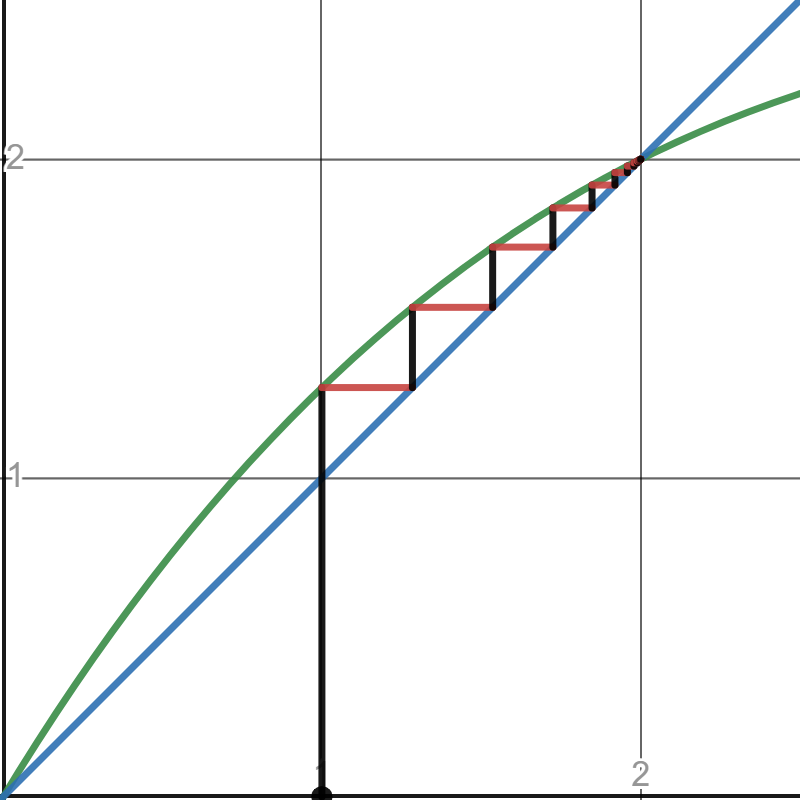
\includegraphics[width=0.4\textwidth]{Ricker_r0.5.png} \quad
            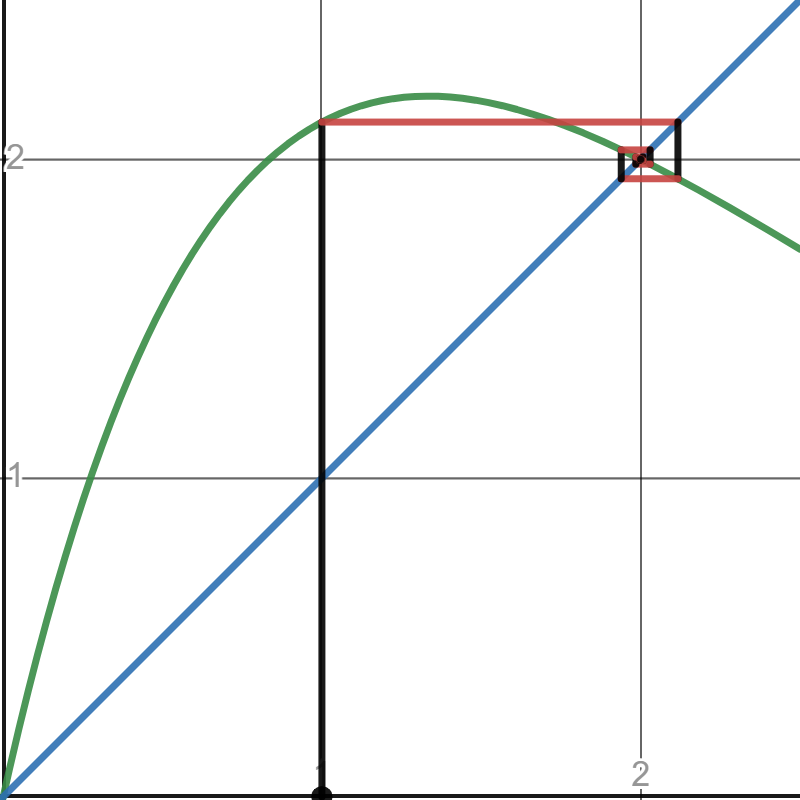
\includegraphics[width=0.4\textwidth]{Ricker_r1.5.png}
        \end{figure}
        
        The two cobweb diagrams are above, with $r=0.5$ on the left and $r=1.5$ on the right. See \href{https://www.desmos.com/calculator/shunsi7ohr}{here} for an interactive version.
        }
        \commentary{Generally done well, but there were a few issues, where one or more of the below points was absent. Full credit was given if:
        
        \begin{itemize}
            \item You said that trajectories approached monotonically for $0 < r < 1$ and oscillatorily for $1 < r < 2$;
            \item You drew the correct \emph{nonlinear} curve (not a linear one) alongside the line $u_{n} = u_{n-1}$;
            \item You labelled the axes (and ideally the curves as well), or it was otherwise very clear what you were drawing and why.
        \end{itemize}
        }
    \end{enumerate}
    \item \textbf{Systems of Difference Equations}
    Now let's consider a simple predator-prey system of the form,
    \begin{align}
        u_n &= ru_{n-1}\exp(-av_{n-1}),\\
        v_n &= u_{n-1}\left(1-\exp(-av_{n-1})\right),
    \end{align}
    where $r>0$ and $a>0$ are positive parameters.
    
    \begin{enumerate}
        \item Determine the equilibria of this model, and state any conditions for each equilibrium to be permissible. NB: You can neglect equilibria which only exist for special single values of parameters (e.g. $r=1$).
        \sol{
        The equilibria are found from the equations,
        $$
        u^* = ru^*\exp(-av^*), \quad
        v^* = u^*\left(1-\exp(-av^*)\right),
        $$
        from which we see one solution as $u^*=v^*=0$, which is always permissible. To find others we can divide the first equation by $u^*$ to find,
        $$
        1 = r\exp(-av^*) \implies v^* = \frac{\ln{r}}{a}.
        $$
        Substituting this into the second equation we find,
        $$
        u^*=\frac{r\ln(r)}{a(r-1)}.
        $$
        The solution above for $v^*$ is only permissible if $r>1$, hence we need this condition for the second steady state to be permissible at all.
        }
        \commentary{Most answered well, but there were a few algebra errors which propagated into the remainder of the questions. Make sure to read carefully and clearly describe any conditions for permissibility. State this even if it is `obvious', i.e.~in the case $(u^*, v^*) = (0,0)$ note that it is always permissible etc.}
        \item Determine the stability of each equilibrium. \emph{Hint:} Remember that the trace and determinant of a matrix can be related to the sum and product of its eigenvalues respectively. That is, $\det(\m{J}) = \lambda_1\lambda_2$ and $\tr(\m{J})=\lambda_1+\lambda_2$.
        \sol{
        As usual, we first find the Jacobian matrix by computing partial derivatives. This gives us,
        $$
        \m{J}(u^*,v^*) = \begin{pmatrix} re^{-av^*} & -aru^*e^{-av^*}\\
        1-e^{-av^*} & au^*e^{-av^*}
        \end{pmatrix}.
        $$
        Evaluation this at the extinction steady state we find,
        $$
        \m{J}(0,0) = \begin{pmatrix} r & 0\\
        0 & 0
        \end{pmatrix},
        $$
        which has eigenvalues $\lambda=0,r$. Hence this equilibrium is stable for $r<1$, and unstable for $r>1$.
        
        For the second equilibrium, we note that $e^{-av^*}=1/r$. Using this, we have,
        $$
        \m{J}(u^*,v^*) = \displaystyle \begin{pmatrix} 1 & \displaystyle-\frac{r\ln(r)}{r-1}\\
        \displaystyle \frac{r-1}{r} & \displaystyle \frac{\ln{r}}{(r-1)}
        \end{pmatrix}.
        $$
        Analyzing the eigenvalues of this matrix in general is difficult. However, using the hint we know that 
        $$
        \det(\m{J}) = \frac{\ln(r)}{r-1}+\ln{r} = \frac{r\ln(r)}{r-1} = \lambda_1\lambda_2.
        $$
        If the eigenvalues lie within the unit circle (that is, the equilibrium is stable), then we must have 
        $$
        |\det(\m{J})| = \left|\frac{r\ln(r)}{r-1} \right|=|\lambda_1\lambda_2| \leq |\lambda_1||\lambda_2| < 1.
        $$
        If this were true, however, for $r>1$ it would imply that $r\ln{r}<r-1$, and as these functions are equal at $r=1$ it would mean this inequality was preserved by taking derivatives, so that $1+\ln{r} < 1$, which is not true for $r>1$. Hence we must have that the positive equilibrium is unstable for all $r>1$, and so always unstable.
        }
        \commentary{A number of mistakes:
        
        \begin{itemize}
            \item Some students did not describe what happens to the extinction equilibrium as $r$ crosses 1 (some students did not analyze $r<1$ as the other equilibrium was not permissible, but $r<1$ is still important to check for stability for this equilibrium);
            \item Some issues remembering how discrete stability is different to ODE stability. Remember that it is no $\Re{\lambda}=0$ that is the stability boundary, but $|\lambda| = 1$!
            \item Computing the eigenvalues is hard, and not easy to determine stability directly; the hint was meant to make it clearer that stability can be determined without computing eigenvalues directly.
        \end{itemize}}
        \item Is this a biologically realistic model? Justify your answer. Can you suggest ways to improve this model?
        \sol{
        The model seems to be well-behaved for $r<1$, giving predictions similar to other models we have seen that the populations die out. However, for $r>1$, the model predicts only unstable solutions, and there are never any stable coexistence regimes. Related to this, in the absence of predators, the prey population grows without bound. Hence this is likely not a good model. 
        
        There are a number of improvements one could make to the model which might help improve stability. A key one would be to add some kind of density-dependent saturation to the prey's response, so that it cannot grow without bound in the absence of predation. In fact, it turns out this leads to a much more realistic model, though one which is harder to analyze without using a computer. See \textsc{Murray}, vol.~I, Section 3.10 for more details.
        }
        \commentary{A few common issues on this question:
        
        \begin{itemize}
            \item Some students did not give a suggested improvement, which was asked for;
            \item Lots of vague waffle (`populations depend on each other'). Try and be clear and precise mathematically when you make claims, such as that the model represents a predator-prey interaction;
            \item There was evidence of terms which appeared from outside the course which didn't make sense in context. It is OK to look things up or use AI, but please ensure you understand what you are saying;
            \item A helpful hint is to look at past problem sheets/problem class sheets/lecture notes to try and get an idea of what `good' interpretation answers look like. Come talk to the lecturers to help too!
        \end{itemize}}
    \end{enumerate}
\end{enumerate}

    
\end{document}